\documentclass[12pt,a4paper]{article}
\usepackage{titlesec}
\usepackage{fancyhdr}
\usepackage{cite}
\usepackage[utf8x]{inputenc}
\usepackage{ragged2e}
\usepackage{amsmath}
\usepackage{float}
\usepackage{graphicx}
\usepackage{algorithm}
\usepackage[noend]{algpseudocode}
\usepackage[parfill]{parskip}
\usepackage{booktabs}
\usepackage{array}
\usepackage{paralist}
\usepackage{verbatim}
\usepackage{subfig}
\usepackage[toc,page]{appendix}
\graphicspath{ {./Images/} }

\pagestyle{fancyplain}
\fancyhf{}
\renewcommand{\headrulewidth}{0.5pt}
\renewcommand{\footrulewidth}{0.5pt}
\setlength{\headheight}{15pt}
\fancyhead[L]{Glenn Wilkie-Sullivan - 40208762}
\fancyhead[R]{ SOC10101 Honours Project}
\fancyfoot[L]{}
\fancyfoot[C]{\thepage}

\makeatletter
\renewcommand\subsection{\@startsection {subsection}{1}{2mm}
                               {3pt plus 2pt minus 1pt}
                               {3pt plus 0pt}
                               {\normalfont\bfseries}}
\makeatother
\makeatletter
\renewcommand\section{\@startsection {section}{1}{0mm}
                               {4pt plus 2pt minus 1pt}
                               {4pt plus 0pt}
                               {\bfseries}}
\makeatother

\makeatletter
\def\BState{\State\hskip-\ALG@thistlm}
\makeatother

\renewcommand{\algorithmicforall}{\textbf{for each}}

\begin{document}

\newcommand{\HRule}{\rule{\linewidth}{0.5mm}}

\begin{titlepage}
	\begin{center}

	\HRule \\[0.4cm]
    	{\Large \bfseries A Comparison of Effectiveness Between Different Representations of Agent Cognitions Using Evolutionary Algorithms\par}
	\vspace{0.2cm}
	\HRule \\[1.5cm]

	
    	\vspace{3cm}
	\begin{minipage}{0.4\textwidth}
	\begin{center} \large
        \emph{}\\
        	Glenn Wilkie-Sullivan - 40208762
				
   	 \end{center}
    	\end{minipage}
	
	\vspace{2cm}
    	\begin{minipage}{1\textwidth}
    	\begin{center} \large
        
		Submitted in partial fulfilment of \\
		the requirements of Edinburgh Napier University \\
		for the Degree of \\
        	BSc (Hons) Games Development
    	\end{center}
    	\end{minipage}

    	\vfill

    	% Bottom of the page
	\begin{minipage}{1\textwidth}
    	\begin{center} \large
		School of Computing
    	\end{center}
    	\end{minipage}
	
	\vspace{1cm}
    	{\large \today}


	\end{center}
\end{titlepage}
%{\large Submitted in partial fulfilment of the requirements of Edinburgh Napier University for the Degree of }

\section*{Authorship Declaration}
\vspace{0.5cm}
\begin{flushleft}
I, (Insert Name eg. Norman Stanley Fletcher), confirm that this dissertation and the work presented in it are my own achievement.\newline

Where I have consulted the published work of others this is always clearly attributed;\newline

Where I have quoted from the work of others the source is always given. With the exception of such quotations this dissertation is entirely my own work;\newline

I have acknowledged all main sources of help; \newline

If my research follows on from previous work or is part of a larger collaborative research project I have made clear exactly what was done by others and what I have contributed myself;\newline

I have read and understand the penalties associated with Academic Misconduct.\newline

I also confirm that I have obtained informed consent from all people I have involved in the work in this dissertation following the School's ethical guidelines.\newline
\end{flushleft}

\begin{flushleft} \large
\emph{Signed:} \\
\end{flushleft}

\vspace{.5cm}

\begin{flushleft} \large
\emph{Date:} \\
\end{flushleft}

\vspace{.5cm}

\begin{flushleft} \large
\emph{Matriculation no: }  \\
\end{flushleft}
\pagebreak

\section*{General Data Protection Regulation Declaration}
\vspace{0.5cm}
\begin{flushleft}
Under the General Data Protection Regulation (GDPR) (EU) 2016/679, the University cannot disclose your grade to an unauthorised person. However, other students benefit from studying dissertations that have their grades attached. \newline

\vspace{0.5cm}

Please sign your name below one of the options below to state your preference.\newline
\vspace{0.5cm}

The University may make this dissertation, with indicative grade, available to others.\newline
\vspace{3cm}


The University may make this dissertation available to others, but the grade may not be disclosed.\newline
\vspace{3cm}


The University may not make this dissertation available to others.\newline

\includegraphics[width=0.3\columnwidth]{sig}
\end{flushleft}



\pagebreak

\begin{abstract}
\noindent
Over the course of over 60 years, the field of game theory has been examined comprehensively, in situations where it can be theoretically applied to economic or mathematical problems. This project will attempt to blend the field of game theory with machine learning and evolutionary algorithms in an attempt to apply theory based reasoning to applicable problems and dilemmata, in the hopes that the results will show success and possible applications to multiple other fields of computing.
\end{abstract}
\pagebreak

\tableofcontents
\newpage

\listoftables
\newpage

\listoffigures
\newpage

\section*{Acknowledgements}
Insert acknowledgements here
\subsection*{}
	-
\newpage


\section{Introduction}
Since 1713, game theory has been a prevalent and ever-rising field. Early work saw the introduction of game theory principles into solutions for economic and mathematical problems, yet didn't hit its main strides until the 1920s and 50s with the work of John von Neumann, Merrill Flood, Melvin Dresher and John Forbes Nash Jr. Books and academic journals such as, "On the Theory of Games of Strategy" from von Neumann and, "Two-person Cooperative Games" from Nash saw possibilities of game theory having applications in fields outside of economics and mathematics. Subsequently in the same decade as Nash's work, game theory saw its first appearance into fields such as philosophy, psychology and political science. \\
Since then, one of the main advances in game theory was made by Robert Axelrod, with his work on the iterated prisoners dilemma - this is the most popular and instrumental occurence of game theory having application in fields such as artificial intelligence and evolutionary biology. \\
This project is an attempt to combine multiple facets of game theory and artificial intelligence, in hope that the end result will be educational and/or useful to the fields; there is also a goal that the end result will be applicable to video games in some way, either through AI agents or through general design. There are multiple stepping stones within the fields of game theory, mathematics, etc. which need to be examined in order to gain a further understanding of the project, which we will look at in the literature of the field(s).

\subsection{Aims \& Objectives}
In order to carry out the implementation side of this project, a strong understanding of the principles and theory behind game theory and artificial intelligence are required. As they tie into each other in this project, there is also a necessity behind learning how to approach the blending of both fields. As seen in the following section, this project covers a considerable amount of previous work and literature which provides the knowledge and insight required to understand or recreate this project. In the literature review, the topics of game theory, artificial intelligence, neural networks and evolutionary algorithms are explored - through their history, applications and relation to this project. From this knowledge, we can form research questions to focus on, and eventually answer at the end of the project. The second part of this report will cover the application of the theory covered within the literature review, as well as a continuation into original ideas for research, as seen by the research questions. This will entail creating a program, or programs, which can compare the validity and effectiveness of machine learning techniques using a game theory scenario - mainly, the prisoner's dilemma. This applies to the research goals as shown: \\

\begin{enumerate}
  \item Research different models of agent cognition, in particular neural networks and finite state machines.
  \item Implement an evolutionary algorithm that can evolve agents to play a repeated Prisoner's Dilemma, where the representation of the evolving agent strategies can be changed between neural networks and finite state machines.
  \item Test the evolutionary algorithm by recreating existing results from the literature.
  \item Perform experimental analysis to determine how the representation of the agent's strategy changes how easy it is for the evolutionary algorithm to find strategies that give high payoffs, i.e. that play the game well.
  \item Perform additional experiments to determine how robust the results are to changes in the game, e.g. Stag Hunt vs Prisoner's Dilemma. \\
\end{enumerate}

\subsection{Scope \& Limitations}
Within this project, there are various delimiters on quality and timeliness - the project will follow a set 8 month time period, and with this comes a few difficulties when approaching the implementation and documentation of the project. As this project attempts to identify the strengths and weaknesses of machine learning techniques, there has to be an clarification that the implementation operates on limited computational power. This means that certain approaches cannot be taken when implementing the theory of the literature review - numerous papers which are instrumental in the game theory field assume that the application will have infinite processing power. However, this limitation is identified as a research question, soon to come. Secondary to this, the time constraint unfortunately limits the amount of possiblities of further applications to other fields such as video games. While there is a definite possibility of application in this field, this report can only cover the theory behind it, instead of an application or visualisation.

\subsection{Report Structure}
The reader will see that the report structure is systemically approaching the final product of this project - the literature review will examine the ideas and motivation behind the project, as well as foundations for the planning behind the implementation. This includes the approaches that will work, and any limitations the implementation will encounter. Subsequently, the implementation will identify the programming language(s), packages/libraries and environment(s) required to approach the planning of the project, and then how the final program looks in execution. The results and evaluation section will then cover the strengths and possible downfalls of this product, what went right and what went wrong. This allows any reader to recreate the approaches of the project while avoiding any problems encountered in this section. This section will also contain the comparison of effectiveness between machine learning techniques, and foundations to conclude on which approach is better or worse. With this, the project can verify its integrity and robustness, then conclude and answer the research questions posed at the beginning, which can be seen in the following section.

\newpage

\section{Literature Review/Background}
\subsection{Brief History of Game Theory}
Game theory is the study of behaviours and mathematical models which result from the decisions and strategies of two or more economically rational players in either cooperative or non-cooperative strategy games. Applications of game theory have manifested in social science, psychology, mathematics and many more fields of study; however, the root interactions lie in strategic games such as the prisoner's dilemma or tit-for-tat. Game theory was introduced and popularised by mathematician John von Neumann, who first proved an optimal strategy for zero-sum games with perfect information such as chess or go called the minimax theorem in 1928. This theorem indicates that in such games, there is a pair of strategies for each player which allows them to minimise their maximum losses, while considering all responsive moves of the opponent. \\
\noindent
After von Neumann published his initial paper on game theory, he published a book co-authored by economist Oskar Morgenstein entitled, "Theory of Games and Economic Behaviour". Within this book, von Neumann fixates mainly on non-cooperative games and/or zero-sum games; but most importantly, identified a method of finding consistent solutions and strategies for both players in two-person zero-sum games. This work became a milestone for game theory as it established a foundation for becoming a unique discipline. \\
\noindent
Following this, numerous advancements in game theory occurred during the 1950s - mathematicians Merrill Flood and Melvin Dresher experimented mathematical and game versions of the prisoner's dilemma for the American think tank corporation, RAND (Research and Development). In the same year, John Forbes Nash Jr published his dissertation on non-cooperative games which contained the first definitions of the Nash equilibrium - an important milestone for adaptive strategy in game theory. He proved that in every n-player non-zero sum game, a Nash equilibrium existed, assuming the game had a finite number of actions. This was a continuation of the work from von Neumann and Morgenstein in their 1944 book, which only covered two person zero-sum games, and was restrained by the implications of 'rational' behaviour. \\
\noindent
In 1980, political scientist Robert Axelrod set up a multi-agent tournament for the iterated/repeated prisoner's dilemma. Multiple well-known game theorists from different professions such as psychology, political science, economics, mathematics and more submitted 14 FORTRAN (Formula Translation) programs for the agents to follow as implicit strategies. In this tournament, agents would play against each other for 200 rounds - mutual cooperation would yield 3 points, mutual defection 1 point, single defection 5 points and single cooperation 0 points. The winning strategy was a simple tit-for-tat program which cooperated on the first turn, then repeated the opponents previous move for each subsequent turn. This strategy ended the tournament with an average of 504.5 points of a maximum 1000. \\

\subsection{Prisoner's Dilemma}
The prisoner's dilemma is one of the fundamental games of game theory which shows the payoffs and consequences of two 'players' acting in their own self interests. This summary, cited from britannica.com, is a model version of the prisoner's dilemma: \\

\noindent
"\textit{Two prisoners are accused of a crime. If one confesses and the other does not, the one who confesses will be released immediately and the other will spend 20 years in prison. If neither confesses, each will be held only a few months. If both confess, they will each be jailed 15 years. They cannot communicate with one another. Given that neither prisoner knows whether the other has confessed, it is in the self-interest of each to confess himself. Paradoxically, when each prisoner pursues his self-interest, both end up worse off than they would have been had they acted otherwise.}" \\

\noindent
The first examples of the prisoner's dilemma being used in the context of game theory date back to the 1950s, by Merrill Flood and Melvin Dresher who devised puzzles and experiments using the structure of the dilemma - mainly an attempt to verify the usefulness of a non-cooperative Nash equilibrium. In this experiment, Flood and Dresher ran 100 games between two human players - in which player 1 (economist Armen Alchian) cooperated 68 times, while player 2 (mathematician John Williams) cooperated 78 times. In game theory, if a strategic game exists with the possibility for a various number of possible outcomes, a payoff matrix can be used to visually represent the benefits and consequences of each outcome. For the prisoner's dilemma, a typical payoff matrix would look as such:

\begin{figure}[h]
	\centering
		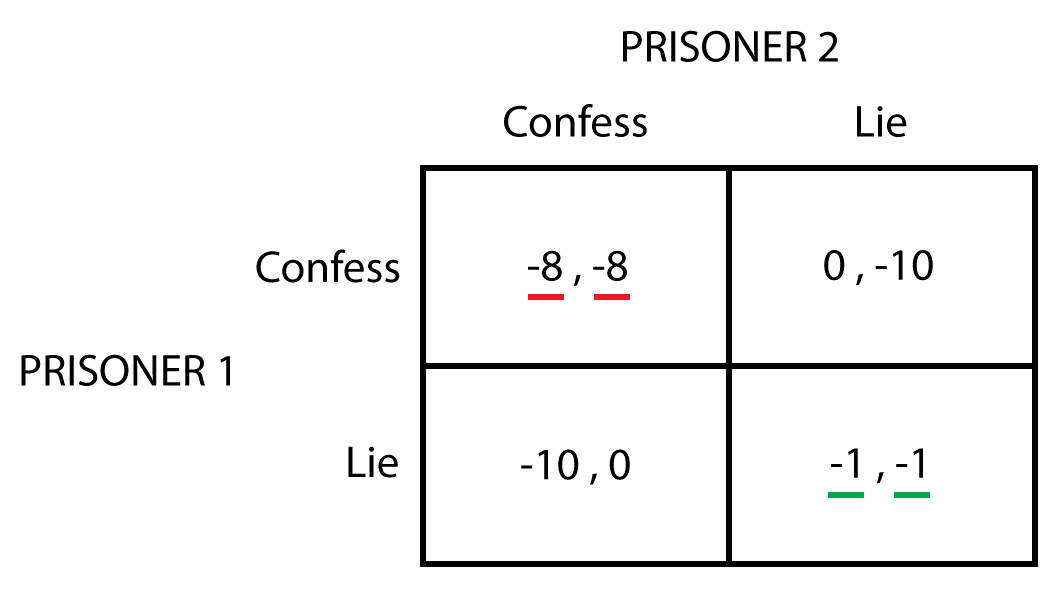
\includegraphics[width=0.6\textwidth]{DilemmaPayoffMatrix}
		\caption{Prisoner's Dilemma Payoff Matrix}
\end{figure}

\noindent
As you can see, the prisoner's would achieve the best possible equal payoff if they consistently chose to confess, but a prisoner could achieve a higher payoff if they were to follow their own self interests. However, the payoff matrix in this experiment looked like this:

\begin{figure}[H]
	\centering
		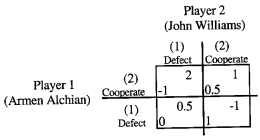
\includegraphics[width=0.5\textwidth]{FloodDresherPayoff}
		\caption{Flood-Dresher Experiment Payoff Matrix (de Herdt, 2003, p. 184)}
\end{figure}

\noindent
In the Flood-Dresher experiment, the restraints can be thought of as 'unfair' as human players have a level of empathy and other emotion which may sway their decision for reasons an A.I. program would never follow. Such an example would be the comments which player 1 made in their log of comments. Alchian, or player 1, wrote comments such as "He does not want to trick me. He is satisfied. I must teach him to share", while player 2 Williams wrote comments such as "A shiftless individual - opportunist, knave" (de Herdt, 2003, p. 189) just a turn apart from each other. Many economists, game theorists and mathematicians believe that the results of this experiment may have been swayed slightly due to each player being empathetic or vindictive at numerous points in the game. \\

\subsection{Nash Equilibrium}
In 1950, John Forbes Nash Jr. published his dissertation entitled, "Non-cooperative Games". Within this dissertation was proof which indicated that within a two person zero-sum game, there exists an 'equilibrium point' for both players. This equilibrium was described in the paper as such, "Thus an equilibrium point is an n-tuple such that each player's mixed strategy maximizes his pay-off if the strategies of the others are held fixed. Thus each player's strategy is optimal against those of the others" (Nash, 1950, p. 3). Simply put, Nash was illustrating that within a two person game in which one player's benefit is a direct loss for the opponent, there lies a state in which neither player has any incentive to switch strategies, as it will not benefit their payoff - thus, the game sits at an equilibrium. The simplest, and most likely quickest way to prove the existence of a Nash equilibrium would be as follows:

\begin{figure}[H]
	\centering
		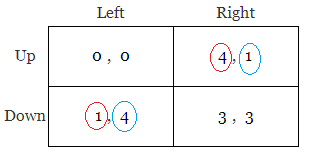
\includegraphics[width=0.5\textwidth]{ModelMatrix}
		\caption{Example Matrix}
\end{figure}

\noindent
Most proofs of equilibria exist if a certain number of conditions are met. Given a model payoff matrix, figure 3, our conditions for a pure/mixed strategy Nash equilibrium are as follows:

\begin{itemize}
  \item The first player's best response is the same against any potential move of the opponent (red circle).
  \item The second player's best response is the same against any potential move of the opponent (blue circle).
  \item Nash equilibrium = (Up, Right),(Down, Left).
\end{itemize}

\noindent
There are a few ways of proving the existence of a Nash equilibrium within games in a more detailed way - within Nash's dissertation, he chose to speak about the 'generalised' Kakutani fixed point theorem, and the Brouwer fixed point theorem. The Kakutani theorem is a more generalised proof of the Brouwer fixed point theorem, but is used to prove a Nash equilibrium in a very similar way. The conditions used in both theorems can be modified in such a way that you would prove the existence of an equilibrium state rather than a fixed point, within a set of strategies rather than tuples.

\subsubsection{Applications of Game Theory}
Beside its obvious magnitude in the fields of mathematics, Nash's work has had effects on fields such as computing, social science, psychology, and many more. Economists have used examples of the Nash equilibrium to calculate the prices of rival companies, predict prices of future products and calculate the best prices for supply and demand. A dissertation/report was published by the federal reserve bank of Minneapolis looking into why car insurance was so expensive in Philadelphia in the 90s, in which the writer chose to use a Nash equilibrium to demonstrate why the fluctuation of price was caused by the rivaling strategies of insurance providers. However, given the unpredictability of today's market, a Nash equilibrium may not have many uses outside of being a mathematical model in the field of economics. Another famous example would be the Cold War between the 40s and 90s - the USSR and the US were stuck in a long period of tension which could be seen as mutually assured destruction, in which each bloc knew the positions of the opponent but didn't start a war. This correlates exactly to a Nash equilibrium situation, where each side has no incentive to switch their strategy given the payoff.  Aside from it's obvious applications in machine learning, game theory has appeared in subfields of computer science such as social networks, recommender systems and resource managers. Similarly, in the field of video games, game theory is becoming more prevalent - specifically in games where strategic decision making is involved, such as Firaxis Games' 'Civilization VI' or Ensemble Studios' 'Age of Empires'. In these games, it is entirely possible, and quite likely that players will end up in situations similar to the prisoner's dilemma or even a Nash equilibrium due to its resource management and turn-based system. In a 2-player game of Civilisation VI, both players have the possibility of knowing where the other's resources (soldiers/capitals/units) are, but have a mutual acceptance of not attacking each other (Cooperation). However, at any point in the game, either player could defect from this peace and attack the other in order to increase their payoff, maybe winning the game. In a field such as multi-agent systems, the prisoner's dilemma is a common occurrence when dealing with e-commerce situations such as auctions. For example, an auctioning site such as eBay has the issues of shill bidding and sniping taking over the market. The general process of an auction is a prisoner's dilemma - if the seller is viewed as the judge/prosecutor in the classic dilemma scenario and the buyer is viewed as the prisoner, there is a communication 'grey-area' in which neither side knows the true price of what is being sold, both have an incentive to overcorrect, leading to cooperative and defective choices. \\

\subsection{Repeated Games}
Repeated games, also known as iterated games or 'supergames' are either finitely or infinitely long games which repeat after finishing. These games are usually represented in extensive form, meaning each strategy and/or game is mapped out as a tree, with specific time-stamps for each game. Payoffs are included at the end of each branch. The main application and usefulness of repeated games is to examine how economically rational players may behave differently from game to game depending on previous strategies or moves. Arguably the most important instance of repeated games is Robert Axelrod's multi-agent tournament in 1980. This tournament was a simple 200 round prisoner's dilemma, in which mutual cooperation scored 3 points, mutual defection 1 point, single defection 5 points and single cooperation 0 points - with a 200 round maximum of 1000 points. Well known game theorists from multiple professions such as psychology, political science, economics, mathematics and sociology submitted FORTRAN (Formula Translation) programs which the agents would follow as strategies. The winning strategy was submitted by Professor Anatol Rapoport, which was a simple tit-for-tat program in which the agent would start with a cooperative choice, then mimic the opponent's choice on the previous turn. According to Axelrod in his primer, "This decision rule is probably the most widely known and most discussed rule for playing the Prisoner's Dilemma. It is easily understood and easily programmed" (Axelrod, 1980, p. 7). Interestingly, each participant of the tournament was made aware of the properties of the preliminary tournament, and thus, many of them made tit-for-tat programs which they tried to improve upon; but, the original and simple tit-for-tat program ended up performing better than the modified versions. In relation to this project, FORTRAN would not be applicable/feasible to use, given its dependency on supervision (previous data or knowledge). Essentially, this means that it is incredibly difficult to evolve individual, high-level lines of code from non-functional languages such as FORTRAN, Java, C\# and so on. Evolutionary algorithms essentially make random changes - thus, if this was replicated with random changes to lines of code in an imperative language, the program would undoubtedly become unstable or not work. The same can be said for any attempts to 'evolve' lines of code like an evolutionary algorithm. As a subsitute to this, the project will use neural networks and finite state machines to evolve a strategy, as both methods are reliable, efficient and have the capability to easily 'evolve'. Another interesting approach to this project would be to use Lisp, another high-level language which is functionally similar to FORTRAN. \\
Within the tournament there were 3 strategies which were expected and known by the participants in advance - always defect, always cooperate, and random. A strategy in which the agent always defects is the safest strategy of any, and could be seen as a principle of game theory. However, although such a strategy is safe, there is a low chance of it being the best strategy due to it's 'no risk, no reward' drawback. The 'always cooperate' strategy performs well when matched against itself - as you can expect a maximum payoff, but when matched against a defecting opponent, there comes a minimum payoff. The 'random' strategy is simply cooperating 50\% of the time, in an attempt to reap the benefits of both strategies. This strategy is more of a utility for making sure the opponent's strategy accounts for all possibilities, but in the end the random strategy didn't perform well. Scores for these strategies can be seen in figure 4.

\begin{figure}[H]
	\centering
		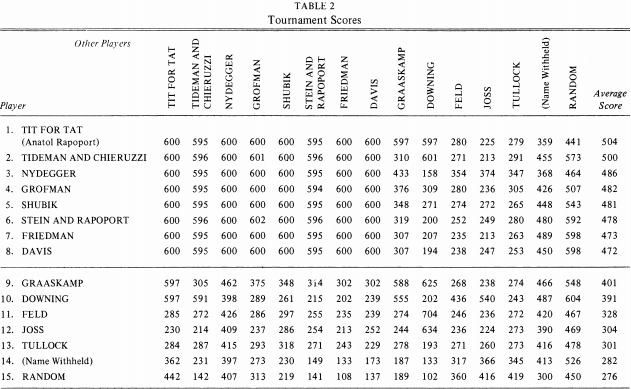
\includegraphics[width=0.7\textwidth]{AxelrodTournamentScores}
		\caption{Scores from the Axelrod Tournament (Axelrod, 1980, p. 11)}
\end{figure}

\subsubsection{Folk Theorem}
Folk theorem is used within repeated games to show that a Nash equilibrium outcome in a game which is repeated infinitely is quantitatively and qualitatively equal and rational to that of a single game. While the origin of this theorem is unknown, it appeared in the 1950s and was quickly spread through the game theory field - thus the name, Folk Theorem. The first instance of a research paper to use the theorem was authored by James W. Friedman (1971) in his article, "Non-cooperative Equilibrium for Supergames", in which he details the payoffs of subgame-perfect \footnote{A subgame-perfect equilibrium means that if players were playing a smaller game which was part of a bigger game, their behaviour would represent a Nash equilibrium of that smaller game.} Nash equilibria in an infinitely repeated game, instead of using a single Nash equilibrium. This means that within a game such as the prisoner's dilemma, where mutual defection is a Nash equilibrium, folk theorem allows the possibility of a non-defection Nash equilibria in infinitely repeated games. Another important concept of folk theorem is that of duopolies and oligopolies; in an economic circumstance, a duopoly is a point in which two suppliers own all or nearly all of the market for a product or service. An oligopoly is the same, except the number of suppliers is more than 2 but remains a small number. When applied to the prisoner's dilemma, any choice other than mutual defection is unstable - however, if the games are infinitely repeated, there exists a possibility that one player may 'threaten' the other player to defect, in which case they would always play defect from that point onwards. In such a situation, if the second player is aware of this threat, they may choose to collude with their opponent and play cooperate, assuming there is a beneficial payoff guaranteed. In both economics and game theory, you can see a riskier, higher payoff as 'discounted' when colluding. Given that scenarios using the folk theorem are infinitely repeated, there are possibities of replicating the results with an indefinitely-long game, as long as there was a high chance of success that an agent would follow the same strategy. As a final thought in reference to Axelrod's tournament, it is confusing that Axelrod didn't consider or even mention folk theorem in his findings. Given the structure of the tournament, there are definite foundations for subgame Nash equilibria, which would've made for interesting comments from Axelrod on the value of specific equilbria at various points of the tournament. \\

\subsection{Machine Learning}
Machine learning is a subfield of articifical intelligence which combines pattern recognition and computational learning theory, an idea pioneered by Alan Turing in 1950, and developed by Arthur Samuel in 1959 through his paper, "Some Studies in Machine Learning Using the Game of Checkers''.\footnote{While some may argue that Marvin Minsky pioneered the first instance of a self-learning machine in 1951, many still question whether or not this project was artificial intelligence, given the amount of missing information.} The main goal of machine learning is for algorithms to become `smarter' on each iteration of instructions, such as a move in a game of checkers, to then make predictions based on the data it has constructed. Within Samuel's introduction to his paper, he states, "The studies reported here have been concerned with the programming of a digital computer to behave in a way which, if done by human beings or animals, would be described as involving the process of learning" (Samuel, 1959, p. 1). Samuel's checkers algorithm used a search tree to identify each of the board positions reachable from the available pieces\footnote{Samuel described this process as `looking ahead a few moves' like a human player might do.}, which would feed into a scoring algorithm - incorporating von Neumann's minimax strategy to choose the best move. The result of this algorithm, through rigorous testing, was a piece of artificial intelligence which could, "greatly outperform an average person'', and was envisioned to be economically viable in real-life situations/problems. This is the first instance of an algorithm which has developed itself without being given information directly. Since the 1950s, machine learning has become almost ubiquitous; in Pat Langley's paper, "Applications of Machine Learning and Rule Induction'', he shows applications of machine learning in over 15 different fields - such as economics, insurance, astronomy and more. Given the two main methods of learning, supervised and unsupervised, only unsupervised learning is applicable to this project. Supervised learning requires prior data in order to predict patterns; Instead, representations of cognitions will be used, as explained in the following section(s). The algorithm will eventually learn and get better with each generation, which is unsupervised. \\

\subsection{Evolutionary Algorithms}
Evolutionary algorithms, or evolutionary computation, is a facet of artificial intelligence in which an algorithm filteres through a set of data, removing the least fit values within a specified iteration, while keeping the most fit values until better values are found. The first appearance of a theory for automated problem solving originated in the 1950s, while application for said theory was developed in the following decade by Lawrence J. Fogel. Fogel devised the idea of evolutionary programming while working for the National Science Foundation, when he saw the approach to heuristic algorithms and primitive neural networks simulations as limited. He theorised that in order for artificial intelligence to progress, the approaches to simulating behaviour should be focused on evolution and increasing intellect rather than model human behaviour. Primarily, "Fogel considered intelligence to be based on adapting behavior to meet goals in a range of environments" (De Jong, 2014, p. 2). This meant that simulated experiments using a finite state machine could be used to investigate intelligent behaviours in a range of situations, with certain rules in consideration. Upon experimenting and publishing multiple papers on the topic, Fogel described, at a very general level, behaviour as the composite ability to predict one's environment, and thus adapt/respond to it suitably. According to Kenneth De Jong of George Mason University, Fogel made a similar proposal for a finite-state machine to replicate this behaviour to that which follows: \\

\noindent
"\textit{A population of finite-state machines is exposed to the environment, that is, the sequence of symbols that have been observed up to the current time\footnote{For the sake of generality, the environment was described as a sequence of symbols taken from a finite alphabet.}. For each parent machine, as each input symbol is offered to the machine, each output symbol is compared with the next input symbol. The worth of this prediction is then measured with respect to the payoff function (e.g. all–none, absolute error, squared error, or any other expression of the meaning of the symbols). After the last prediction is made, a function of the payoff for each symbol (e.g. average payoff per symbol) indicates the fitness of the machine.}" \\

\noindent
The general process involved picking a 'best' or best-suited machine to predict new symbols in the environment, and then the process is repeated until the payoffs can't increase any further, relative to the accuracy (or worth) of their previous predictions. Further work on this research in fields such as sequence prediction, pattern recognition and gaming was conducted by academics such as Bernard Lutter and Ralph Huntsinger (1968), Akihiro Takeuchi (1980) and many others.

\noindent
Since these first occurrences of evolutionary programming, many strides have been made in the field - taking it in a number of directions such as neural network training, image processing and general computing optimisation. Within the facet of neural networks, foundational and important work comes from researchers such as Peter Angeline in 1994 with his paper on evolutionary algorithms and neural networks, J.R. McDonnell and D. E. Waagen's paper on evolving recurrent perceptrons, and Vincent Porto's paper on alternative neural network training methods. In Angeline's paper, he explains why the previous methods of constructing/modifying neural networks are limited - Timur Ash authored a paper on dynamic node creation, but Angeline outlines that only feedforward networks work in application (which isn't effective as a standardised method).\footnote{A feedforward neural network is an artificial neural network wherein connections between the nodes do not form a cycle.} Another researcher of neural networks, Scott Fahlman, authored a paper explaining a recurrent version of the Cascade-Correlation learning architecture in the context of neural networks, but assumes a restricted form of reccurence according to Angeline, which limits the types of input/output, and is generally less robust. A version of the cascade-correlation learning architecture can be seen as follows: \\

\noindent
\begin{figure}[H]
	\centering
		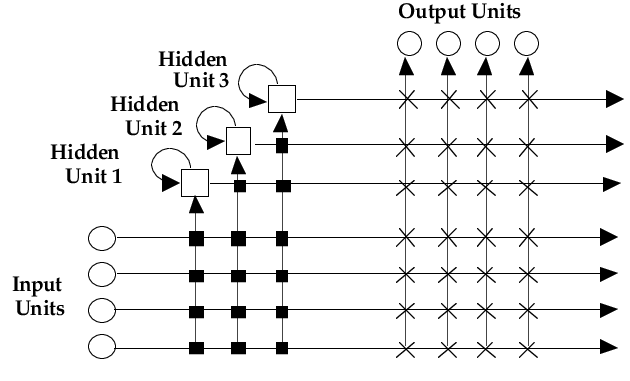
\includegraphics[width=0.7\textwidth]{CascadeCorrelationLearningArchitecture}
		\caption{Cascade Correlation Learning Architecture}
\end{figure}

\noindent
Finally, Dong Chen authored a paper on the constructive learning of recurrent neural networks with the help of C.L. Giles, G.Z. Suna, H.H. Chen, Y.C. Lee and M.W. Goudreaub. However, Angeline explains that the paper only explores fully connected topologies (in which all nodes are connected), without accounting for any other possibilites. Considering these limitations, Angeline presents GNARL (GeNeralized Acquisition of Recurrent Links),  "a network induction algorithm that simultaneously acquires both network topology and weight values while making minimal architectural restrictions and avoiding structural hill climbing" (Angeline, 1996, p.2). This is essentially an evolutionary algorithm which is 'better suited' for evolving neural networks as opposed to genetic algorithms, as it has the boone of function optimisation and the ability to fit a variety of tasks/problems. Angeline then goes on to detail the process of evolving neural networks with both genetic and evolutionary algorithms, and eventually his own `GNARL' algorithm, which "nonmonotonically constructs recurrent networks to solve a given task". Essentially, this algorithm decides the number of input and output nodes relative to the task it has been given, and the number of hidden nodes can range from 0 to whatever the user specifies - avoiding the limitations of the previous work mentioned before.

\noindent
Following this work, one of the next milestones to occur in the field of evolutionary algorithms was the work of J. R. McDonnell and D. E. Waagen. This paper was centered around providing an alternative to feedforward networks for 'nonlinear models of time-series data', by creating the s imple parts of evolutionary algorithms and neural networks in a more efficient and effective way, so that they can be applied to more complex structures or networks. Specifically, the authors decided that, "Once feasibility is demonstrated for simple recurrent perceptron structures, the evolutionary search method can be applied to highly recurrent perceptron networks with complex architectures" (McDonnell; Waagen, 1994, p. 1). This is an interesting way to look at this topic as it can be applied to a large number of tasks/problems, given that the method doesn't address a specific topology - such as stochastic, recurrent or hierarchical. Pseudocode for a generic evolutionary algorithm can be seen as follows: 

\begin{algorithm}[H]
\caption{Basic Evolutionary Algorithm}\label{euclid}
\begin{algorithmic}[1]
\Procedure{GeneticAlgorithm(S - set of blocks)}{}
\State $\textit{Initialisation()}$
\State $t \gets \textit{0}$
\State $\textit{Initialise P$_t$ with random individuals from S*}$
\BState \emph{Evaluate-Fitness-GA(S, P$_t$)}:
\While {\textit{termination condition not met}}
\State {\textit{Select values from P$_t$ (fitness proportionate)}}
\State {\textit{Recombine individuals}}
\State {\textit{Mutate individuals}}
\State {Evaluate-Fitness-GA(S, \textit{modified individuals})}
\State ${\textit{P$_{t+1}$} \gets \textit{newly created values}}$
\State ${\textit{t} \gets \textit{t + 1}}$ \linebreak
\Return (\textit{Superstring derived from best individual in P$_t$})
\State \EndWhile
\BState \emph{Evaluate-Fitness-GA(S - set of blocks, P - population of individuals)}:
\State \textbf{foreach} \textit{individual i  ∈  P} \textbf{do}
\State \textit{generate derived string s(i)}
\State $\textit{m $\gets$ all blocks from S that are not covered by s(i)}$
\State $\textit{s'(i) $\gets$ concatenation of s(i) and m}$
\State $\textit{fitness(i) $\gets$ $\frac{1}{||s'(i)||\textsuperscript{2}}$}$
\EndProcedure
\end{algorithmic}
\end{algorithm}

\subsubsection{Artificial Neural Networks}
Artificial neural networks (ANN) are information processing systems based on biological nervous systems such as the brain. Neural networks are a subfield of machine learning as they make decisions and perform tasks based on previous information they have been given, called training examples. Each system has three layers - input, output, and a layer for filtering the input to something which can be used by the output layer. This is possible due to an algorithm called backpropagation (backward propagation of errors), which calculates the gradient of the error function\footnote{The Gauss error function is the integral of the standard normal distribution.} with respect to the weights of the network. When designing a neural network, there are various paradigms or methods which can be used - only one of which is applicable for this project: control tasks. The other being classification, but this requires labeled training data to train the network, which this project will not have. Backpropagation and supervised learning also isn't valid/feasible within this project, as there is no prior training data to filter/modify to the output layer. Control tasks are reward-based behaviours which can train the decision making process of an evolutionary algorithm. With a neural network being the controller in question, a control task would reward correct behaviour as a method of training the network. Classification is the process of grouping similar values within the network based on their attributes/characteristics. Assuming the possbility of a 'noisy' data set at any point during the program lifecycle, this method would allow the network to classify patterns from data which they have not yet been fed/trained.

\subsubsection{Finite State Machines}
Finite state machines, or finite state automaton, are computational models used to simulate sequential logic or solve problems relating to software architecture. At a very basic level, computers can be seen as state machines; each instruction that a computer receives and execute will change it's state in some way, altering the behaviour and causing subsequent actions or allowing further instructions to occur. Arguably the pioneers of finite state machines, the first proposal and description of finite automata came from neurophysiologists Warren McCulloch and Walter Pitts in 1943 with their paper, "A Logical Calculus Immanent in Nervous Activity". Within this paper, McCulloch and Pitts comprehensively cover topics such as neural network theory, the theory of automata and the theory of computation and cybernetics. Around 10 years later, the first implementation of the finite state machine appeared, created by computer scientists G. H. Mealy and E. F. Moore, with their Moore and Mealy machines. The Mealy machine is focused on determining ouput through the input and current state, while the Moore machine bases the output on the current state alone. Another notable paper which covers finite state machines is Matthijs van Veelen and Julián García's paper, "Direct reciprocity in structured populations". Within this paper, van Veelen and García tackle the topic of finite state automata within an 'open-ended, infinite strategy space'. This topic encompasses that, "Our simulations contain a mutation procedure that
guarantees that every finite state automaton can be reached from every other finite state automaton through a sequence of mutations. Thus, every strategy that can be encoded by a finite state automaton is a possible mutant" (van Veelen; García, 2012, p. 9929). This is done because the state machines that require fewer mutations are essentially the best fit. Nowadays, one of the most significant applications of finite state machines is within video games; games ranging from basic like Pacman to incredibly detailed such as Horizon: Zero Dawn (H:ZD) both use finite state machine for their AI agents. In a game such as H:ZD, creatures will start in a state such as 'idle' or 'roaming' to simulate random animal behaviour, but will switch behaviours to something like 'hunt' once a player is spotted. Other important applications of finite state machines include things such as pattern searching in text editors or IDEs, vending machines, or even system/software modelling. \\

\subsection{Research Questions}
Although a lot of content has been created through many years of research into game theory, machine learning and evolutionary algorithms, there are still a lot questions yet to be answered. In this project, I aim to tackle some of these unanswered questions, with topics such as these:

\begin{enumerate}
\item Given the results of research papers in the past such as Nash's, Harrald's or Axelrod's, how do those results look now when used within a model of more realistic computational power?
\item When using different representations of an agents' cognition, how does the payoff vary between evolved strategies from neural networks and finite state machines? How easy is it to evolve those representations at a high payoff?
\item Within an evolutionary algorithm, which neural network topologies are favoured in 2-player games when a neural network is being used as a representation of the agents' cognition(s)?
\item During this project, neural networks will be used with a fixed shape and payoff matrix. If it is allowed to evolve, how does the shape of the neural network change? (Optional) \\
\end{enumerate} 

\subsection{Conclusion}
In summary, we have analysed multiple facets of fields such as game theory, machine learning, neural networks and evolutionary algorithms in terms of their history, use and sometimes applicability to video games and other forms of media. In all cases, each field has some form of possibility for being in video games - machine learning, neural networks and evolutionary algorithms can all be applied to AI agents to improve their realism and general behaviour. Papers from researchers such as Nash, Harrald and Axelrod have avenues of further research, and while there are continuations of said work, there is yet to be solid proof of applications similar to this project. The results of this project will touch on applications to specific facets of video games and possibly computer science which may not have been explored before. Research for this project arguably starts with Nash's paper in the 50s - the existence of the Nash equilibrium was the driving force behind this project, which eventually led me to read more into game theory. This led to papers from researchers such as Axelrod and Harrald; work from these reports was instrumental in aiding my understanding game theory from a theoretical standpoint, but not necessarily from an application standpoint. The next step was to read work from Kakutani and Brouwer, then Flood and Dresher. While the Kakutani and Brouwer papers were helpful in understanding the processes behind finding a Nash equilibrium, the Flood-Dresher paper was helpful in understanding how game theory scenarios can be applied to real life situations.

\noindent
With this knowledge of game theory and the Nash equilibrium in mind, a necessary step was to find ways to apply it in application. The first works to read were that of Fogel, Waagen and Porto. These papers comprehensively covered neural networks, such as their creation, evolution and learning methods. While helpful, it was the later papers from Fogel and works from researchers such as Chen, Ash and Fahlman that solidified my knowledge on the operation of neural networks. However, what was lacking was a comparitive component. Very little, if any, papers did a comprehensive comparison of methods for game theory application, so it seemed beneficial to tackle that exact topic. With a topic in mind, I came across papers from Angeline, van Veelen and Jong which were extremely useful for learning the history and applications of both machine learning and evolutionary algorithms - another possible method of game theory application. I had to find more papers to read to make sure that a comparison of finite state machines and neural networks within evolutionary algorithms was a fair avenue of research, which led me to papers from Samuel, Lutter and Huntsinger, and Langley. This finalised my understanding of how to approach the project, as well as possible research questions, which you can see above. This project will be an amalgam of the knowledge gained from all of these papers, in an effort to tackle the questions which previous papers did not ask or answer.

\newpage

\section{Methodology}
%Within this section, the general approach to the planning program(s) will be covered, as well as the motivation and reasoning for the research goals and questions.
As discussed previously, a working knowledge of game theory, machine learning and evolutionary algorithms is required to implement the base dilemmata of classic game theory scenarios. In the following section, the required knowledge will be comprehensively examined - such as game theory terms, associated technologies and operations of artificial intelligence architectures. \\

\subsection{Approach}
To have a robust and intensive implementation of the proposed ideas, a selection of milestones and criteria must be met to execute the goals of the project. Before attempting said implementation, the end result of the project must be abstracted into clearer and easier-to-understand points which will be clarified as follows. First, in order to simulate a game theory scenario, a program must be created which can support two agents, represented as both neural networks or finite state machines - playing against each other in a game determined through a payoff matrix as discussed previously. Following this, an evolutionary algorithm must be used to progress the game and evolve the agents through summation of payoffs and fitness functions. Assuming these facets are working as intended, the program should now be able to play a repeated prisoners' dilemma game, all the while evolving the agents to become better/fitter as the game progresses. The variables associated with the neural networks/finite state machines and the evolutionary algorithm should be modifiable to recreate results of research papers conducted previously, such as, ”Evolving continuous behaviors in the Iterated Prisoner's Dilemma” by Harrald in 1996. With this done, the topic of the dissertation can be tackled - assuming there are multiple working versions of the program discussed previously; using both finite state machines and neural networks as representations of the agents' cognitions, both methods can be compared and evaluated based on their use of computation power, difficulty, ease of use and overall suitability. The remainder of this section will cover all of the knowledge required to understand these milestones - such as the general terminology used, program structure and explanation of milestones. \\

\subsection{Technologies}
In order to execute these milestones, a suitable method of application must be identfied. For this project, the implementation of the proposed ideas will use the Python programming language, which will be touched on in a following subsection. Multiple integrated development environments (IDE) exist for Python such as PyCharm, created by the Czech company, Jetbrains, and Spyder (Scientific PYthon Development EnviRonment), created by Pierre Raybaut. This project will be executed using Spyder, given its overall suitability for theoretical and scientific programming.

\subsubsection{Python}
The forementioned programming language, Python, is a high-level, interpreted language developed by Guido van Rossum in 1991 which can utilise multiple programming architectures such as the object-oriented, imperative, functional and procedural paradigms. Given its overall versatility, general abstraction and library support, Python seems more suited than other languages such as C++ or Java for the task(s) at hand. To aid the process of implementation, the NEAT library will be used to handle network creation and management.

\subsubsection{NEAT}
According to their official website, “NEAT (NeuroEvolution of Augmenting Topologies) is an evolutionary algorithm that creates artificial neural networks”. NEAT was developed by Kenneth O. Stanley in 2015 and upheld by the group, CodeReclaimers. The purpose of NEAT in context of this project is to initialise a population of agents, contain and handle the attributes associated with them and control the speciation between rounds of the game. In some games such as the prisoners' dilemma, speciation is not applicable and will be turned off. NEAT also has the functionality of visualising various facets of the game, such as population size per generation, or fitness per generation.

\subsubsection{Python Development Environments}
Integrated development environments (IDE) are software applications which aid program creation, offering tools such as a source code editor, build automation tools, and a debugger. Programs can be compiled, tested and executed by simply clicking a run button, as opposed to compiling the code manually through the command line, respective of your operating system. In relation to Python specifically, a number of open-source (free) IDEs exist. Within these are PyCharm, PyDev, Spyder and many others. Each IDE differs in what it offers, usually suiting a particular type of task. PyCharm is specifically aimed at new Python developers, offering easy Python installations and useful documentation pages on various facets of the program. Conversely, Spyder is aimed at adept Python developers, offering a number of scientific libraries in the base installation package, as well as easy library inclusion for advanced functions. With that in mind, Spyder was justifiably the best platform for the project development. \\

\subsection{Terminology}
When discussing the program in following sections, a range of different technical terms will be used - some of which have been used but not explained in previous sections.

\subsubsection{Agents}
In this facet of programming, an agent is a term used to represent a code structure which makes seemingly logical decisions. In the prisoners' dilemma scenario used within this project, an agent will represent each prisoner, in the effort to emulate a real world scenario in which the agents play against each other. Each agent/prisoner will have a fitness, which could be compared to a real-world aptitude or ability. They will also have a particular strategy, in comparison to real-world, economically rational thinking.

\subsubsection{Fitness Function}
Within an evolutionary algorithm, a fitness function will calculate the quality of a solution to a given problem. The algorithm will find the best input value for the fitness function, and select with of the solutions are the most adequate for the scenario. In this case, the fitness function will sum the payoffs of each agent for every round, and use the eventual value as the new fitness. The results will detail what moves the agents have chosen on average.

\newpage

\section{Implementation and Testing}
In this section, the program structure and content will be covered, as well as a measure of its intuitiveness and robustness. The final program can be compared to the original concept in the methodology section.

\newpage

\section{Results}
After implementing the program, this section will hold discussions regarding the output of the program - whether it is correct or not, as well as comparisons between the various experiments of the project. A discussion of results could cover the following examples:

\begin{itemize}
  \item Comparison of fitnesses between finite state machines and neural networks.
  \item How many generations for each technique to reach the desired result?
  \item How do the results vary when certain variables are changed? e.g population size, number of rounds, mutation/crossover size.
  \item After their strategy is evolved, do the agents ever reach a point in which they always defect? This is an indicator that the program output is correct.
  \item How do the results change between different game theory scenarios?
  \item How complicated are the best strategies?
\end{itemize}

These discussions may be followed or preceded by visualisations of the results.

\newpage

\section{Evaluation}
In comparison to the original plans of the project, i.e implementation and testing, what would be done differently if the project were re-attempted? This section will cover the rigour of the approaches and how well they may/may not have paid off. This may involve comparisons of approaches at the end of the project vs. the start. In addition, there will be discussions on how the output of the program(s) compare to previous research from Harrald, Axelrod, etc.

\newpage

\section{Conclusion}
After covering the previous sections, what can be taken away from this project? The research goals and questions must be revisited in order to answer whether or not they were achieved. There may also be possible discussions on further research.  

\newpage
\bibliographystyle{apalike}
\bibliography{bib}{}
\nocite{*}

\newpage
\begin{appendices}
\section{Initial Project Overview (IPO)}
\textbf{Initial Project Overview} \\
\newline
\textbf{SOC10101 Honours Project (40 Credits)}\\
\newline
\textbf{Title of Project: Learning to Play: Nash Equilibria in Repeated Games Using Machine Learning and Neural Networks} \\
\newline
\textbf{\underline{Overview of Project Content and Milestones}} \\
\newline
The aim of the project is to investigate how changing the representation of an agent's cognition changes how easy or difficult it is to evolve effective strategies for playing repeated games. \\
\newline
The key milestones to achieving this are:
\begin{enumerate}
  \item Research different models of agent cognition, in particular neural networks and finite state machines.
  \item Implement an evolutionary algorithm that can evolve agents to play a repeated Prisoner's Dilemma, where the representation of the evolving agent strategies can be changed between neural networks and finite state machines.
  \item Test the evolutionary algorithm by recreating existing results from the literature.
  \item Perform experimental analysis to determine how the representation of the agent's strategy changes how easy it is for the evolutionary algorithm to find strategies that give high payoffs, i.e. that play the game well.
  \item Perform additional experiments to determine how robust the results are to changes in the game, e.g. Stag Hunt vs Prisoner's Dilemma. \\
\end{enumerate}

\textbf{The Main Deliverable(s):}
\begin{enumerate}
  \item The main deliverable of the project is to have a robust program which houses an evolutionary algorithm capable of handling both finite state machines and neural networks, as forms of representations of an agents’ cognition within a repeated game theory scenario. These agents should be able to play against each other in multiple games, with evolving strategies. These representations should be able to evolve, whether they be controllers such as neural networks or finite state machines.
  \item The secondary deliverable will be an experimental analysis into the controllers of the program: neural networks and finite state machines. When these techniques are implemented within the program, they must be compared to identify the best method of evolving an agents’ strategy/cognition by ways of algorithm fitness or strategy payoff. \\
\end{enumerate}

\textbf{The Target Audience for the Deliverable(s):} \\
\newline
The finished product of the project will most likely require some working knowledge of game theory and/or machine learning to understand. Ideally, the finished product will have enough of an interesting result to yield possibilities of further research, which may interest those with experience in the applicable fields. \\

\textbf{The Work to be Undertaken:} \\
\newline
The project will first require a great amount of research and review. Most of the foundational work applicable to this project was published in the 1950s/60s, with important work on evolutionary algorithms and neural networks between then and the present. Thus, most of the information needed for the project is a collection of professional papers and/or publications written by well-established mathematicians and game theorists. \\
A system will need to be designed and implemented to sustain 2 agents, a repeated game scenario, a neural network and a relay of information which the agents can train from. This system will all be built in the Python programming language - and may use code packages as reference material. \\
After a suitable system is designed and implemented, the user should have control over the power of computation for the agents, and the weights/payoffs of the neural network should be serialised to a CSV file – which can used to compare results between iterations of the games. \\
The end result of the project should have the ability of experimentation, although the best strategies should more or less be the same/similar on each iteration depending on the situation. Ideally, the project should be able to replicate the results of the iterated prisoner’s dilemma experiment by Harrald and Fogel in 1996, if given the same initial values. \\

\textbf{Additional Information / Knowledge Required:} \\
\newline
I will be honing my skills in Python and project management. I will ideally have a working knowledge of artificial intelligence, machine learning and evolutionary algorithms. Additionally, I will learn about the various packages and features of Python which are applicable to the project. \\

\textbf{Information Sources that Provide a Context for the Project:} \\
\newline
Work leading up to the eventual discovery of the Nash equilibrium was authored by John von Neumann and John Forbes Nash. Work on repeated games was introduced and popularised by Robert Axelrod. Work on neural networks was arguably pioneered by Marvin Lee Minsky with his creation of the SNARC (Stochastic Neural Analog Reinforcement Calculator). \\

\textbf{The Importance of the Project:} \\
\newline
From a personal standpoint, the project will be important for gaining useful information on topics I’ve never studied, and the end result will hopefully be a proud accomplishment which I can show to employers. If said result is good enough, the project itself may be a useful research topic/experiment for others in the future. The project as a whole should also be a good investigation tool into how much computation power is needed for a project of this type, as this project will have limited power. These results should be helpful in answering the question of whether or not these scenarios can be adapted to evolve non-player characters in video games. \\

\textbf{The Key Challenge(s) to be Overcome:} \\
\newline
There is an inevitable difficulty when dealing with these topics – game theory, artificial intelligence and evolutionary algorithms are difficult fields to put into application, and I suspect there will be an inherited difficulty which comes with the task. Blending such fields may prove difficult given the free open-source software, in which work like this project may/may not have been done before. Finally, given the time and effort constraints of university, the timelines and workloads other modules may make it difficult to complete each deliverable on time. \\

\section{Interim Report Overview}
Insert a copy of the project review form you were given at the end of the review by the second marker

\section{Diary Sheets \& Project Management Documents}
\textbf{\textit{September}}
\newline
\hrule
\textbf{\underline{Week 1}} \\
\newline
\textbf{Objectives:} \\
The initial goal of the meeting was to examine and modify the first draft of the initial project overview document, with the hope of improving it to a standard for submission. 
Another goal was to discuss the project timeline, and how it should be laid out in a chart. \\

\textbf{Progress:} \\
Upon reading the draft of the document, Simon discussed and agreed suitable goals/milestones of the project, which would eventually be placed into a project timeline chart (Gantt). Simon and I then made changes to a couple of sections in the IPO document, then discussed plans for how the program should be designed. This led to Simon proposing an unofficial, rough change of the project title, given the new scope of design and implementation: “Learning to play: A comparison of effectiveness between different representation of agent cognitions using evolutionary algorithms and machine learning”. Simon also suggested reading up on evolutionary algorithms, as well as emailing the new second marker as per my prompt. \\

\textbf{Goal for Next Week:} \\
Finish IPO document, refine for submission. \\
Finish project timeline (Gantt Chart). \\

\textbf{\underline{Week 2}} \\
\newline
\textbf{Objectives:} \\
The goal of this meeting was to finalise the initial project overview document, as well as establish clear milestones for the project and iron out any concerns I had since the last meeting. \\

\textbf{Progress:} \\
Simon suggested multiple changes to the initial project overview document in order to have it ready for submission, mainly to do with the aims/deliverables of the project. Simon and I then agreed realistic dates for the deliverables, as well as what was expected at each point. We then sorted out a Github collaboration issue and discussed how the project timeline should be laid out.  \\

\textbf{Goal for Next Week:} \\
Finish the evolutionary algorithms section of the literature review. \\
\hrule

\textbf{\textit{October}}
\newline
\hrule
\textbf{\underline{Week 3}} \\
\newline
\textbf{Objectives:} \\
The goal of this meeting was to scan over the literature review of the project, so that Simon could see the structure and overall content quality and eventually offer feedback for each section. I also had to iron out a few queries/thoughts regarding the referencing and citation facet of the project. \\

\textbf{Progress:} \\
Simon started by looking over the list of references for the literature review to make sure they were all in the correct format and reliable sources. He then suggested a few papers to read and then add to the list, as a good general reference for the review such as books/papers by John Maynard Smith and Ken Binmore. After this, Simon started to read over the content of the literature review, and offered a number of suggestions/changes for the benefit of quality/readability. \\

\textbf{Goal for Next Week:} \\
Finalise first draft of the literature review, to eventually look over the content. \\

\textbf{\underline{Week 4}} \\
\newline
\textbf{Objectives:} \\
The goal of this meeting was to comprehensively edit and finalise the literature review based on Simon’s feedback, as well as draft research questions for the project to focus on. \\

\textbf{Progress:} \\
Simon started by looking over the research questions I drafted, suggesting things to add and things to remove. After editing the research questions down to 3, we moved on to editing the literature review. Simon suggested a large amount of changes, in order to get the review fit for submission. \\

\textbf{Goal for Next Week:} \\
Start looking at implementation, maybe bring a basic first demo. \\

\textbf{\underline{Week 5}} \\
\newline
\textbf{Objectives:} \\
The goal of this meeting was to go over progress for the week. \\

\textbf{Progress:} \\
Simon looked over the changes I made to the literature review for the past week to make sure they were all good for the review. He then suggested a few final edits, which finalises the literature review. \\

\textbf{Goal for Next Week:} \\
Implement an evolutionary algorithm which can evolve a neural network, then demo. \\

\textbf{\underline{Week 6}} \\
\newline
\textbf{Objectives:} \\
The goal of this meeting was to go over progress for the week regarding neural networks/evolutionary algorithms implementation. \\

\textbf{Progress:} \\
Simon started by looking over the reference material I found to check if it was applicable. He explained why the implementation of this project isn’t similar to the other repositories and how it should look. Simon suggested reading up on the operation of neural networks – specifically Haykin’s book.  \\

\textbf{Goal for Next Week:} \\
Read on the operation of neural networks, make sure understanding of implementation is solid. \\
\hrule

\textbf{\textit{November}}
\newline
\hrule
\textbf{\underline{Week 7}} \\
\newline
\textbf{Objectives:} \\
The goal of this meeting was plan the implementation of the project. \\

\textbf{Progress:} \\
Simon suggested a good amount of tips for how to approach the program, and what the eventual output should be.   \\

\textbf{Goal for Next Week:} \\
Work on implementation – neural networks + evolutionary algorithms. \\
\hrule

\newpage
\section{Original Proposed Project Timeline}

\begin{figure}[H]
	\centering
		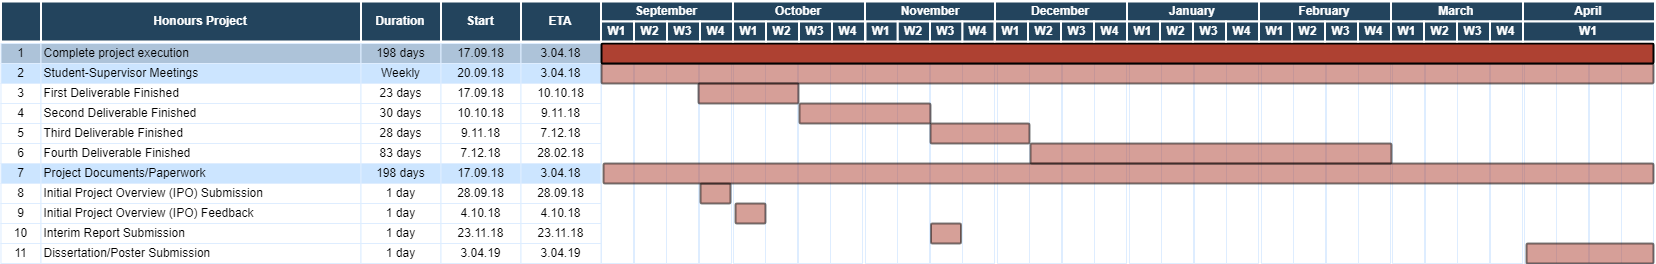
\includegraphics[width=1.5\textwidth,height=\textheight,keepaspectratio, angle=90,origin=c]{HonoursTimeline}
\end{figure}

\end{appendices}

\end{document}
